\begin{Example}[icu1]{Survival in the ICU}
In this example we examine briefly some aspects of logistic regression
related to model selection and graphical display with a mixture of
quantitative and discrete variables.
We use data from a study by
\citet{Lemeshow-etal:88}
of patients admitted to an intensive care unit at
Baystate Medical Center in Springfield,
Massachusetts.  The goal of this study was to develop a
model to predict the probability of survival (up to hospital
discharge) of these patients and to study the risk factors associated with 
ICU mortality.
Data for a sample of 200 subjects from this study are given in
\citet[App. 2]{HosmerLemeshow:89}, and reproduced in
\datref{dat:icu}.

There are 19 explanatory variables, of which three (age, systolic blood pressure and heart rate) are quantitative, one is categorical (race),
and the remaining 15 are binary (many having been dichotomized).
Initial model screening was carried out using the forward, backward,
and stepwise procedures using the \opt{SELECTION}{LOGISTIC}
on the \stmt{MODEL}{LOGISTIC}.  As in other model selection procedures,
it is prudent to regard these simply as ``candidate'' models,
nominated for further attention. 
The results for the full model with
all 19 predictors and for the final selection models are shown below.

\begin{center}
 \begin{tabular}{l rrrrr p{5.5cm}}
 \hline
  Selection & AIC & SC & $G^2$ & Score & df & Variables in Model \\ 
  \hline
  Full model & 160.78 & 226.74 & 79.38 & 74.74 & 19 & All \\ 
  Stepwise & 149.14 & 165.63 & 61.03 & 62.67 & 4 & Age Cancer Admit Uncons \\ 
  Forward & 149.14 & 165.63 & 61.03 & 62.67 & 4 & Age Cancer Admit Uncons \\ 
  Backward & 144.44 & 170.83 & 71.72 & 70.52 & 7 & Age Cancer Admit Uncons Systolic pH PCO \\ 
 \hline
 \end{tabular}
\end{center}

For the moment, we focus on the variables Age, Cancer, Admit
(elective vs.\ emergency admission) and
Uncons
(stupor or coma at admission).  These were nominated by all three procedures, and 
constitute the best model according to the forward and stepwise
procedures.  Estimated coefficients and odds ratios for this model
are shown in \outref{out:icu1.1}, fit using the statements below.
The lack of fit test (output not shown) gives $\chisq (8) = 5.081, p=0.74$,
showing no evidence of need for a more complex model.
\begin{listing}
%include data(icu);
proc logistic data=icu nosimple order=data;
     model died = age  cancer  uncons admit /
           scale=none aggregate lackfit;
     output out=results p=predict l=lower u=upper / alpha=.33;
\end{listing}

\begin{Output}[htb]
\caption{ICU data: Parameter estimates}\label{out:icu1.1}
\small
\verbatiminput{ch6/out/icu1.1}
\end{Output}
Because age is continuous, it is sensible to plot predicted
results against age, and to construct separate curves according
to the combinations of the other risk factors which are present
for each case.   A  composite variable \pname{risk} is created
combining the values of Cancer, Admit, and Uncons which all correspond
to increased risk of death.
\begin{listing}
data results;
   set results;
   length risk $16;
   if cancer then risk = 'Can';
   if admit  then risk = trim(risk) ||' Emerg';
   if uncons then risk = trim(risk) ||' Uncon';
   if risk =' ' then risk='None';
   risk = left(risk);
   label predict='Estimated Probability of Death';

proc sort;
   by risk age;
\end{listing}
The following steps create Annotate labels for the risk factors
and plot predicted probability of death for each combination,
producing the graph in \figref{fig:icu11}.
%% one figure
\begin{figure}[htb]
  \centering
  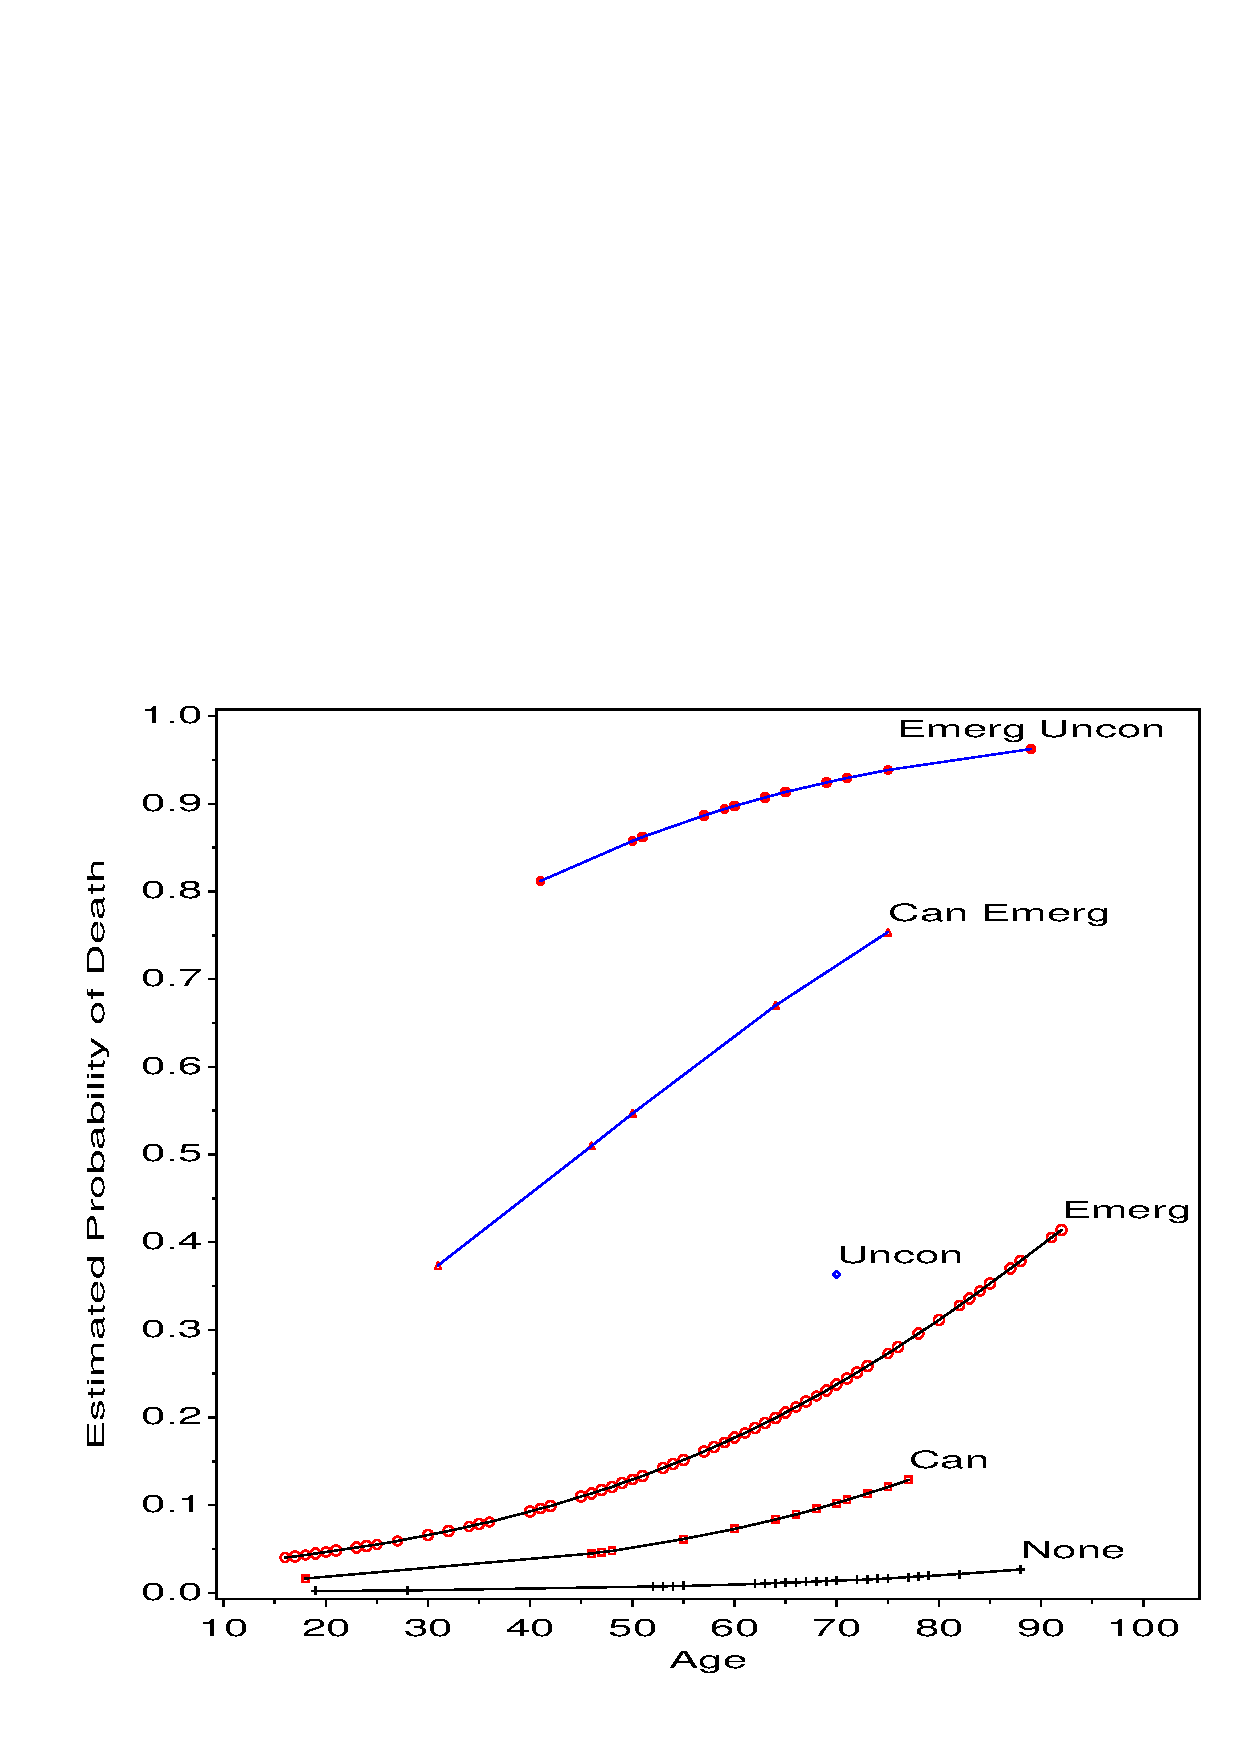
\includegraphics[scale=.6]{ch6/fig/icu11}
  \caption[ICU Survival data: Predicted probabilities]{ICU Survival data: Predicted probabilities for combinations of risk factors vs.\ age}%
  \label{fig:icu11}
\end{figure}
\begin{listing}
data label;
   set results;
   by risk;
   retain xsys ysys '2';
   position ='3';
   if predict>.9 then position='2';
   if last.risk then do;
      x = age;  y=predict;
      function = 'label   ';
      text=risk;
      output;
      end;

proc gplot data=results;
   plot predict * age = risk /
      frame anno=label vaxis=axis1 haxis=axis2 vm=1 hm=1 nolegend;
   axis1 label=(a=90);
   axis2 offset=(,4);
   symbol1 i=join v=square   c=red ci=black;
   symbol2 i=join v=triangle c=red ci=blue;
   symbol3 i=join v=circle   c=red ci=black;
   symbol4 i=join v=dot      c=red ci=blue;
   symbol5 i=join v=plus     c=black;
   symbol6 i=join v=diamond  c=blue ci=blue;
 run; quit;
\end{listing}
From the graph, it is apparent that mortality increases with
age when any of these risk factors are present, particularly
when the patient is admitted to Emergency; it is highest when the
patient is also unconscious at admission.  
From the odds ratios (see \outref{out:icu1.1}), we see that the
odds of death are increased 40-fold when the patient is unconscious.
The graph, however, shows the effects of these risk factors in
combination, and also indicates the number and age distribution of cases which have these combinations.

Before concluding that this model provides an adequate description of the
data, we should examine whether any individual cases are unduly influencing
the predicted results, and more importantly, the choice of variables in
the model.  We examine this question in \secref{sec:logist-infl}
where we return to these data (\exref{ex:icu2}).
\end{Example}